\chapter{重症医学科获得性感染与感染控制}

\section{前沿学术综述}

过去10年中,严重感染发生率增加了91.3%,并以每年1.5%~8.0%的速度上升。虽然器官支持技术及抗感染治疗取得长足进步,但感染性休克患者病死率仍高达30%~70%,是重症患者最主要的死亡原因。

\subsubsection{重症医学科获得性感染的流行病学}

重症患者由于器官功能衰退、侵入性操作较多、免疫屏障破坏以及抗菌药物反复使用等容易发生院内感染,一旦发生院内感染病死率明显增高。院内感染的主要类型为呼吸机相关性肺炎、血管内导管相关血流感染、导尿管相关尿路感染、腹腔感染、切口感染等,其中以三管(气管导管、血管内导管、导尿管)引发的感染为重症医学科院内感染监控的重点和感染检查的必查项目。

院内感染的致病菌种近年来逐渐发生变迁。以导管相关血流感染为例,以往导致导管相关血流感染的病原菌主要为凝固酶阴性葡萄球菌、金黄色葡萄球菌、肠球菌等,且耐药菌占很大比例,如耐甲氧西林的表皮葡萄球菌、耐甲氧西林的金黄色葡萄球菌和耐万古霉素的肠球菌等。近年来,耐甲氧西林的金黄色葡萄球菌引起的导管相关血流感染有所减少,可能与手卫生等预防措施的实施有关
\protect\hyperlink{text00031.htmlux5cux23ch1-30}{\textsuperscript{{[}1{]}}}
\textsuperscript{,}
\protect\hyperlink{text00031.htmlux5cux23ch2-30}{\textsuperscript{{[}2{]}}}
;而耐三代头孢和碳青霉烯的革兰阴性菌和耐氟康唑的念珠菌在逐渐增多。最近疾病控制中心的统计数据显示,引起导管相关血流感染的病原菌中革兰阴性杆菌可达20%以上。另外,以往铜绿假单胞菌在院内革兰阴性菌感染中占第一位,而近来不动杆菌、尤其多重耐药的鲍曼不动杆菌感染明显增多,在重症医学科院内感染中明显高于铜绿假单胞菌。因此需建立各医院或科室的流行病学资料,以指导感控的管理和重症感染的早期经验性治疗。

\subsubsection{重症医学科获得性感染的防治进展}

近年来重症患者多重耐药菌所致的严重感染明显增加,成为当前重症患者抗感染治疗面临的重大挑战。对于院内感染,尤其是多重耐药菌感染,预防非常重要。严格的手卫生和单位隔离有利于减少耐药菌的传播。对于各种导管相关感染(导管相关血流感染、呼吸机相关性肺炎、导尿管相关尿路感染等)国内外均制定了相应的预防指南或集束化治疗策略,并在不断更新
\protect\hyperlink{text00031.htmlux5cux23ch3-30}{\textsuperscript{{[}3{]}}}
\textsuperscript{,}
\protect\hyperlink{text00031.htmlux5cux23ch4-30}{\textsuperscript{{[}4{]}}}
。如对于导管相关血流感染,2011年国际上推出最新的预防指南,提出导管置入和感染控制的集束化治疗策略,为临床血管内导管的管理提供了更加详细科学的指导。

早期有效的抗菌药物治疗能够明显降低严重感染及感染性休克的病死率。研究显示,若在严重感染发生低血压后1小时内应用广谱抗生素治疗,患者的生存率高达79.9%,但抗生素应用每延误1小时,存活率降低7.6%。由此可见早期、准确、有效抗生素应用对于严重感染和感染性休克的治疗是至关重要的。目前临床主要依据美国胸科学会指南提出的多重耐药菌感染高危因素进行多重耐药菌感染的筛查,并进行早期抗感染治疗
\protect\hyperlink{text00031.htmlux5cux23ch5-30}{\textsuperscript{{[}5{]}}}
。但新近研究发现,按照美国胸科学会指南进行预测重症患者入重症医学科时是否为多重耐药菌细菌感染,其阳性预测值仅为18%,假阳性率高达82%,提示美国胸科学会指南对多重耐药菌细菌定植及感染存在明显局限,可能导致抗生素的不必要使用,产生抗生素选择性压力诱导的细菌耐药,而早期病原微生物的携带筛查,有助于弥补美国胸科学会指南的不足,成为早期有效合理使用抗菌药物治疗的前提和基础。通过筛查患者转入及转出重症医学科的细菌携带情况,记录患者是否具有多重耐药菌定植或感染的高危因素,有助于明确重症患者多重耐药菌的流行病学特征,从而为多重耐药菌感染的早期合理抗生素治疗提供重要依据。而周期性的对病区环境、医护人员手部的病原菌筛查,有助于明确院内感染的传播途径,制定和采取有效的措施减少和控制院内感染、尤其是多重耐药菌导致的感染的发生。

病原菌的主动筛查包括以下内容:①入住重症患者的常规筛查,包括留取咽拭子、痰、血、分泌物以明确是否已携带多重耐药菌病原体;②对重症医学科环境和物品,如呼吸机、监护仪、呼吸囊、空气等进行定期标本培养,尤其在病区院感爆发时进行监测;③对医护人员的手部进行拭子培养,明确手卫生情况以及判断病原菌是否经手传播。

对于检出多重耐药菌细菌,且确定为感染而非定植或污染,则需要进行抗菌治疗。抗菌药物的目标性选择需根据药敏和病情严重度而定。近期针对重症医学科常见的不动杆菌推出《2011中国鲍曼不动杆菌感染诊治与防控专家共识》,为临床不动杆菌的防治提供了很好的参考
\protect\hyperlink{text00031.htmlux5cux23ch6-30}{\textsuperscript{{[}6{]}}}
。

\subsubsection{重症医学科获得性感染的问题与前景}

对于院内感染,尤其是重症医学科内各种导管引发的感染产生的费用问题,在国外已有明确规定,如美国联邦医疗保险与医疗救助服务中心规定,自2008年10月1日后出院的患者,如出现导管相关血流感染、导尿管相关泌尿系感染等八类情况,将不再支付给医院相关费用。在美国,导管相关血流感染控制目标为“零容忍”。在我国,目前尚无明确的限定值,但已作为重症医学科质量控制的指标之一和感控检查的重点。国家已开始建立健全全国医院感染监控网络,通过不断反馈与比较,相信不久的将来必定会出台各种导管相关感染率的控制目标。

多重耐药菌的防控与清除是重症医学科院内感染控制中的难点,除持续的手卫生监控外,设备的消毒也非常重要。很多院感的爆发与设备的污染相关。在国外,当一名患者转出后,其床边所有的仪器设备都将移出进行彻底的消毒。但在国内限于空间和经济的限制,在设备消毒方面仍存在很大欠缺,也是院内感染发生和爆发流行的潜在危险,有待于不断改善。

耐药菌的产生与抗菌药物的不合理使用有直接关系。2011年4月7日为第60个世界卫生日,其主题是:“抵御耐药性:今天不采取行动,明天就无药可用。”自2011年起,卫生部已对各级医院的抗菌药物种类进行了限制,并颁发了相应的抗菌药物临床应用管理规范,并督导医疗过程中的具体执行情况。反复的培训和抗菌药物合理使用的不定期检查将有助于改善抗菌药物滥用的现状。

\section{临床问题}

\subsection{重症医学科患者院内获得性感染概述}

\subsubsection{什么叫院内获得性感染,常见类型有哪些?}

院内获得性感染是指住院患者在入院48小时后获得的感染,包括在住院期间发生的感染和在医院内获得出院后发生的感染,但不包括入院前已开始或者入院时已处于潜伏期的感染。医院工作人员在医院内获得的感染也属医院感染。

常见的类型包括:上呼吸道感染、下呼吸道感染、血源性感染、胃肠道感染、皮肤感染、切口感染、泌尿系感染、腹腔感染、肝炎等。

\subsubsection{院内感染有何严重性?}

院内感染可在患者、医院、社会等各个方面产生不良影响。

(1)患者方面:增加患者的住院费用,延长住院时间,甚至导致患者死亡;导致耐药菌的出现与传播,引起抗菌药物选择压力增大。

(2)医院方面:如院内感染爆发,则需关闭病房,由此可带来巨大的经济损失和不良声誉,可能造成重大的公共影响。

(3)社会方面:美国联邦医疗保险与医疗救助服务中心规定自2008年10月1日后出院的患者,如出现以下八类情况,将不再支付给医院相关费用:①手术留下异物;②空气栓塞;③配血不合;④导尿管相关尿路感染;⑤压疮;⑥导管相关血流感染;⑦手术部位感染------冠状动脉搭桥术后纵隔感染;⑧医院内获得的外伤------骨折、脱臼、颅脑损伤、挤压伤、烧伤等。在我国,目前尚无明确的规定,但已将各种导管相关感染的发生率作为重症医学科质量控制的指标之一和感控检查的重点。

\subsubsection{重症患者院内获得性感染有哪些危险因素?}

重症患者由于病情重,多种有创性操作,反复抗菌药物使用,免疫力低下,更易发生医院获得性感染,且较难控制。常见的危险因素有患者个体因素和医源性因素两大类。

常见的患者个体因素包括:免疫功能低下、病情危重(休克、大出血、重大手术、多脏器功能衰竭)、严重的多发性创伤、原发病、营养不良、年龄、药物影响等。

医源性因素包括:长期使用各类抗菌药物使细菌耐药、各种侵入性操作(机械通气、动静脉置管测压、血液净化、静脉营养、留置尿管、胃肠引流等)、危重患者缺乏或丧失自理能力、与护理人员频繁接触引起的交叉感染等。

\subsubsection{重症医学科院内感染的常见部位及病原菌是什么?}

重症医学科的院内感染常见部位以呼吸道为主,其次为血液、泌尿系、胃肠道、手术切口及皮肤黏膜等。其中三管的感染,即导管相关血流感染、呼吸机相关性肺炎和导尿管相关泌尿系感染为临床监控的重点。

感染致病菌以革兰阴性菌为主,其次为革兰阳性菌和真菌,其中耐药菌感染比例高,如耐甲氧西林的金黄色葡萄球菌、耐万古霉素的肠球菌、产超广谱β-内酰胺酶的肠杆科细菌、多重耐药菌铜绿假单胞菌和鲍曼不动杆菌等。

近年来,病原学也在不断发生变迁。以导管相关血流感染为例,通常导致导管相关血流感染的病原菌为凝固酶阴性葡萄球菌、金黄色葡萄球菌、肠球菌等,且耐药菌占很大比例,如耐甲氧西林的表皮葡萄球菌、耐甲氧西林的金黄色葡萄球菌和耐万古霉素的肠球菌等。近来,耐甲氧西林的金黄色葡萄球菌引起的导管相关血流感染有所减少,可能与手卫生等预防措施实施有关;而耐三代头孢和碳青霉烯的革兰阴性菌和耐氟康唑的念珠菌在增多。最近疾病控制中心的统计数据显示由革兰阴性杆菌引起的导管相关血流感染可达20%。另外,以往铜绿假单胞菌在院内革兰阴性菌感染中占第一位,而近来不动杆菌尤其多重耐药的鲍曼不动感染明显增多,在重症医学院院内感染中占第一位。

\subsubsection{院内获得性感染防控的基本环节是什么?}

院内获得性感染防控的基本环节包括3个方面:①控制感染源。包括外源性的(如感染患者及其分泌物、病原菌携带者)和内源性的(如口咽部胃肠道的反流误吸)。②切断传播途径。传播途径分为接触传播(最常见的方式,有直接和间接之分)、空气传播和呼吸道飞沫传播。对于接触传播需要做好手卫生,必要时戴手套;对于呼吸道飞沫传播则需要戴口罩,而空气传播则需要更强的个人防护措施,如手套、口罩、护目镜、防水围裙、长外衣等,且宜单间隔离,有条件时可置于负压病房。③保护易感人群。管理好周边的患者,尤其免疫功能低下者。提高免疫力、减少有创操作、积极营养支持以及抗菌药物合理使用,将有助于患者避免获得或继发院内感染。

\subsection{医院感染爆发事件报告及处置标准操作流程}

\subsubsection{何谓医院感染爆发,如何上报?}

医院感染爆发是指在医疗机构或其科室的患者中,短时间内发生3例以上同种同源感染病例的现象。

疑似医院感染爆发指在医疗机构或其科室的患者中,短时间内出现3例以上临床症候群相似、怀疑有共同感染源的感染病例;或者3例以上怀疑有共同感染源或感染途径的感染病例现象。

医院感染爆发传播方式包括带菌者传播、交叉感染、空气传播或其他方式。

(1)出现医院感染爆发流行趋势时,临床科室经治医师立即报告科主任,同时报告医院感染管理科,确认后及时报告分管院长,并通报相关部门。

(2)经医院调查证实出现以下情况时,医院应于12小时内报告本市医院感染质控中心、卫生行政部门和疾病控制中心。包括5例以上疑似医院感染爆发以及3例以上医院感染爆发。

(3)当地卫生行政部门接到报告后,应当于24小时逐级上报至省级卫生行政部门。

(4)省级卫生行政部门接到报告后组织专家进行调查,确认发生以下情形的,应于24小时内上报至卫生部。包括5例以上医院感染爆发;由于医院感染爆发直接导致患者死亡;由于医院感染爆发导致3人以上人身损害后果。

(5)发生以下情形时应当按照《国家突发公共卫生事件相关信息报告管理工作规范(试行)》的要求进行报告。包括10例以上的医院感染爆发事件;发生特殊病原体或新发病原体的医院感染;可能造成重大公共影响或严重后果的医院感染。

\subsubsection{医院感染爆发的处置预案是什么?}

(1)临床科室发现3例或3例以上相同感染病例(包括症状相同或病原体相同等),应及时上报感染管理科。

(2)医院感染管理科接到报告后应立即到现场核查,在确认医院感染爆发时应立即报告院领导和上级有关部门。

(3)查找感染源及传播途径,隔离相关患者,加强消毒,必要时关闭病房。

(4)制定控制措施,分析调查资料,写出调查报告,总结经验,制定防范措施。

\subsubsection{医院感染爆发的具体调查步骤是什么?}

(1)成立调查小组,调查小组由分管院长、感染控制人员、医院流行病学专家、感染发生部门科主任及护士长、微生物学专业人员、药物学专业人员、后勤保障部主管等组成。

(2)对医院感染爆发病例进行查看,了解病史、核查实验室检查结果,开展相应的流行病学调查。

(3)进行核实会诊,确认是否为真正的医院感染爆发或流行的存在。

(4)调查感染爆发流行的起始时间及医院感染传播方式,列出潜在的危险因素。

(5)根据调查情况,制定临时控制措施。如隔离感染源或可疑感染源或保护性隔离其他患者等。必要时可采用停止手术或关闭病房等措施。

(6)根据感染爆发或流行的调查和控制情况,实时调整相应控制措施并及时完成调查报告。

(7)调查小组向医院感染管理委员会递交书面报告。

\subsection{院内感染与手卫生}

\subsubsection{对手卫生设施有哪些要求?}

(1)采用流动水洗手,手术室、产房、重症监护室等重点部门应当采用非手触式水龙头开关。

(2)固体肥皂应保持肥皂及皂盒的清洁与干燥;皂液宜使用一次性原装的挤压式液体皂,如使用分装液体皂,容器必须保持清洁,并每周至少消毒一次。皂液有浑浊或变色时应及时更换,并清洁、消毒容器。

(3)提倡使用一次性纸巾,或用干手毛巾(一用一消毒,并干燥),避免造成二次污染。

(4)配备合格的快速手消毒剂,并放置在医务人员便于取用的位置,包括流动使用诊疗车上。

\subsubsection{洗手指征有哪些?}

(1)接触患者黏膜、破损皮肤或伤口前后,接触患者的血液、体液、分泌物、排泄物、伤口敷料之后;

(2)直接接触患者前后及接触不同患者之间;穿脱隔离衣前后;

(3)戴手套前、脱手套后(戴手套不能替代洗手);

(4)进行无菌操作前后,处理清洁、无菌物品之前,处理污染物品之后;

(5)处理药物及配餐前;

(6)手有可见的污染物或者被患者的血液、体液等蛋白性物质污染后。

\subsubsection{如何规范洗手?}

(1)湿手:用水打湿双手;(2)涂皂:取适量皂液涂抹所有手部皮肤;(3)揉搓:认真揉搓双手,按照六步法洗手,时间不得少于15秒(见图\ref{fig25-1});

\begin{figure}[!htbp]
 \centering
 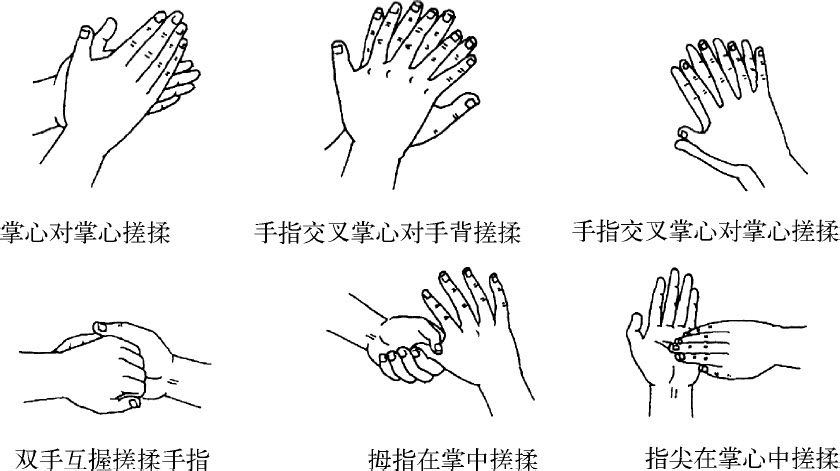
\includegraphics{./images/Image00290.jpg}
 \captionsetup{justification=centering}
 \caption{六步洗手法}
 \label{fig25-1}
  \end{figure} 

(4)冲洗:用流动水冲洗、清洗双手;

(5)干手:用纸巾或干手毛巾干燥双手;

(6)护肤:适量护肤用品护手。

\subsubsection{卫生手消毒的指征和方法有哪些内容?}

卫生手消毒的指征
\protect\hyperlink{text00031.htmlux5cux23ch7-30}{\textsuperscript{{[}7{]}}}
包括:

(1)检查、治疗、护理免疫功能低下的患者之前;

(2)出入隔离病房、重症监护病房等重点部门前后;

(3)需双手保持较长时间抗菌活性时;

(4)为不同患者进行诊疗之间;从同一患者污染部位移动到清洁部位时;手部无明显污染物时;

(5)接触具有传染性的血液、体液和分泌物以及被传染性致病微生物污染的物品后;

(6)双手直接为传染病患者进行检查、治疗、护理或处理传染患者污物之后。

卫生手消毒的消毒方法:

(1)取2~3ml的速干手消毒剂于掌心;

(2)涂抹手的所有皮肤,揉搓方法参照六步洗手法(图\ref{fig25-1}),揉搓时间至少15秒;

(3)揉搓时,保证手消毒剂完全覆盖手部皮肤,直至手部干燥;

(4)符合上述消毒原则第(5)、(6)条者,应先洗手,然后再进行卫生手消毒。

\subsubsection{如何进行外科手消毒?}

(1)卫生用品包括指甲剪、消毒皂液、非手触式清洗液出液器、一次性外科手消毒剂、无菌巾、灭菌洗手刷、计时钟。

(2)外科手术消毒原则:①先洗手、后消毒;②进行各类手术前均应进行外科洗手和外科手消毒;③手术中和不同患者手术之间、手套破损或手被污染时,应重新进行外科洗手和外科手消毒。

(3)外科手清洗、消毒方法 洗手方法:①洗手之前应当先摘除手部饰物,并修剪指甲,长度应不超过指尖;②取适量的清洗液清洗双手、前臂和上臂下1/3,并认真揉搓,清洁双手时,应清洁指甲下的污垢和手部皮肤的皱褶处;③流动水冲洗双手、前臂和上臂下1/3;④使用无菌巾彻底擦干双手、前臂和上臂下1/3。

消毒方法:取适量的免冲洗手消毒剂涂抹双手的每个部位、前臂和上臂下1/3,并认真揉搓直至消毒剂干燥,至少消毒两遍(手消毒剂的取液量、揉搓时间及使用方法遵循产品的使用说明)。

注意事项:①在整个手消毒过程中应保持双手位于胸前并高于肘部,使水由手部流向肘部;②洗手与手消毒双手相互揉搓要充分;③术后摘除外科手套后,应用清洗液清洁双手;④用后的清洁指甲用具、揉搓用品等,应放到指定的容器中;揉搓用品应每人使用后消毒或者一次性使用;清洁指甲用品应每日清洁与消毒。

\subsubsection{洗手能降低多重耐药菌检出率吗?}

院内感染的传播途径以接触传播最常见,手卫生作为院内感染防控中的重要一环,具有直接、简易、经济、有效等优势。但对降低革兰阴性菌和革兰阳性菌多重耐药菌感染的效果有差异。

随着洗手依从性的提高,耐甲氧西林的金黄色葡萄球菌导致的院内感染发生率和导管相关血流感染明显降低。研究表明,经过手卫生干预后,在重症医学科耐甲氧西林的金黄色葡萄球菌引起的定植或感染患者的百分比由9.3/100降至6.7/100,\emph{P}
=0.047;耐甲氧西林的金黄色葡萄球菌导致的血管内导管相关血行感染发生率(千导管日)明显下降(2.0/1000对比1.1/1000,\emph{P}
=0.018
\protect\hyperlink{text00031.htmlux5cux23ch1-30}{\textsuperscript{{[}1{]}}}
。另有研究显示,将洗手依从性从49%提高到98%,耐甲氧西林的金黄色葡萄球菌引发的院内感染发生率从0.52/1000降至0.24/1000
\protect\hyperlink{text00031.htmlux5cux23ch2-30}{\textsuperscript{{[}2{]}}}
。因此,在耐甲氧西林的金黄色葡萄球菌防控指南里明确指出,手卫生作为控制耐甲氧西林的金黄色葡萄球菌的重要一环
\protect\hyperlink{text00031.htmlux5cux23ch8-30}{\textsuperscript{{[}8{]}}}
。

在重症医学科革兰阴性菌院内感染中排在首位的为鲍曼不动杆菌,其为条件致病菌,对湿、热、紫外线、化学消毒剂有较强的抵抗力,在干燥的物体表面可以存活25天以上,常规消毒剂只能抑制其生长,不能杀灭。有大量研究表明,各种仪器设备(如吸引装置、呼吸机、血液净化仪等)可能是导致患者耐药菌传播和院内感染爆发的主要因素。单纯的手卫生可能不能明显控制革兰阴性菌导致的院内感染,尤其是多重耐药菌的鲍曼不动杆菌,单位隔离和加强设备的彻底消毒将有助于阴性菌院感爆发的控制
\protect\hyperlink{text00031.htmlux5cux23ch9-30}{\textsuperscript{{[}9{]}}}
。

\subsection{医院获得性感染防控基本要求}

\subsubsection{在感染控制方面,工作人员如何管理?}

(1)科室工作人员需穿工作服进入科室工作区,应保持服装清洁,每周更换2~3次。接触特殊患者如耐甲氧西林的金黄色葡萄球菌感染或携带者,或经治疗的患者可能出现血液、体液、分泌物、排泄物等污染工作服时,应穿隔离衣。

(2)工作人员接触已有或可能有传染性呼吸道感染患者时,或可能出现患者体液喷溅、进行无菌操作时应戴口罩。

(3)工作人员进入病室需更换清洁的工作用鞋,但不得穿露脚趾的拖鞋。

(4)通常工作人员接触患者时不必戴帽子。无菌操作或可能会有体液喷溅时,必须戴帽子。

(5)工作人员接触患者黏膜和非完整皮肤、进行无菌操作时,须戴无菌手套;接触患者血液、体液、分泌物、排泄物或处理被其污染的物品时,应戴清洁手套。护理患者后要摘除手套,护理不同患者或医护操作在同一患者的污染部位移位到清洁部位时应更换手套。特殊情况下如手部有伤口、给HIV/AIDS患者进行高危操作,应戴双层手套。

(6)严格执行手卫生规范。

(7)科室必须保证有足够的医护人员。医师和护士人数与重症医学科床位数之比必须为0.8~1∶1和2.5~3∶1以上。

(8)工作人员患感冒、腹泻等可能会传播的感染性疾病时,应避免接触患者。

(9)医护人员每年应接受医院感染控制相关知识的培训,卫生保洁人员应接受消毒隔离知识和技能的培训。

\subsubsection{在感染控制方面,患者如何管理?}

(1)应将感染与非感染患者分开安置。

(2)对于疑似有传染性病原体感染或重症感染的患者,应隔离于单独房间。对于经空气传播的感染,如开放性肺结核,应隔离于负压病房。

(3)耐甲氧西林的金黄色葡萄球菌、泛耐药鲍曼不动杆菌等感染或携带者,应有醒目的标识,尽量隔离于单独房间,如房间不足,应将同类耐药菌感染或携带者集中安置。

(4)对于重症感染、多重耐药菌感染或携带者或其他特殊感染患者,应分组护理,固定人员。

(5)接受器官移植等免疫功能明显受损患者,应安置于单间病房且有保护性隔离醒目标识。

(6)医务人员不可同时照顾负压隔离室内的患者和保护性隔离的患者。

(7)如无禁忌证,应将所有患者床头抬高30°。

(8)重视患者的口腔护理。对存在医院内肺炎高危因素的患者,采用洗必泰漱口或口腔冲洗,每日4次。

\subsubsection{在感染控制方面,对访视者如何管理?}

(1)尽量减少不必要的访客探视。

(2)若被探视者为隔离患者,建议穿访客专用的清洁隔离衣。访客着鞋较脏时(如雨天)应穿鞋套。

(3)探视呼吸道感染患者,应戴一次性口罩。对于疑似患有强传染性疾病如禽流感、SARS等的患者,应避免探视。

(4)进入病室探视患者前和结束探视离开病室时,应洗手或用酒精擦手液消毒双手。

(5)探视期间,尽量避免触摸患者周围物体表面。

(6)访客有疑似或证实呼吸道感染症状时,或婴、幼儿童,应避免进入重症医学科探视。

\subsubsection{在感染控制方面,对建筑布局有何要求?}

(1)放置病床的医疗区域、医疗辅助用房区域、污物处理区域和医务人员生活辅助用房区域等,应相对独立。

(2)每个重症医学科管理单元,至少配置1~2个单人房间,用于安置隔离患者。设置病床数量不宜过多,以8~12张床位为宜。尽量多设为单间或分隔式病房。

(3)重症医学科每病床使用面积不得少于15m\textsuperscript{2}
,床间距应在1m以上;单人房间的每床使用面积不少于18m\textsuperscript{2}
。

(4)配备足够的手卫生设施。医疗区域建议每2张床设置一个洗手池,单人房间应设置洗手池。采用脚踏式、肘式或感应式等非手接触式水龙开关,并配备擦手纸等干手设施。每张病床旁须放置手部消毒装置(酒精擦手液)1套。

\subsubsection{医务人员职业暴露预防标准操作流程有哪些方面?}

(1)医务人员在进行侵袭性诊疗、护理、实验操作过程中,要保证充足的光线,并特别注意防止被针头、缝合针、刀片等锐器刺伤或划伤。

(2)禁止将使用后的一次性针头双手重新盖帽,如需盖帽只能用单手盖帽,禁止用手直接接触污染的针头、刀片等锐器。

(3)手术中传递锐器建议使用传递容器,以免损伤医务人员。

(4)使用后的锐器应当直接放入耐刺、防渗透的利器盒中,以防刺伤。

(5)医务人员进行有可能接触患者血液、体液的诊疗、护理和实验操作时必须戴手套,操作完毕,脱去手套后立即洗手或进行手消毒。

(6)在诊疗、护理、实验操作过程中,有可能发生血液、体液飞溅到医务人员的面部时,医务人员应当戴口罩、防护眼镜;有可能发生血液、体液大面积飞溅或者有可能污染医务人员的身体时,还应当穿戴具有防渗透性能的隔离衣或者围裙。

(7)处理污物时严禁用手直接抓取污物,尤其是不能将手伸入到垃圾袋中向下压挤废物,以免被锐器刺伤。

(8)所有被血液、体液污染的废弃物均应焚烧处理。

\subsection{重症医学科患者多重耐药菌携带筛查与监控}

\subsubsection{何为MDR、PDR、XDR}

关于描述耐药菌的几个术语“多重耐药菌(MDR)”,“泛耐药菌(XDR)”和“全耐药菌(PDR)”的定义,国内外尚有些争议
\protect\hyperlink{text00031.htmlux5cux23ch10-30}{\textsuperscript{{[}10{]}}}
。为便于不同医疗机构和国家的流行病学监测数据收集和比较,2010年,美国、瑞典、以色列、希腊、荷兰、瑞士、澳大利亚等国家的一些专家共同提出了关于MDR、XDR、PDR术语国际标准化的建议(草案),并于2012年在ClinMicrobiol
Infect上正式发表
\protect\hyperlink{text00031.htmlux5cux23ch11-30}{\textsuperscript{{[}11{]}}}
\textsuperscript{,}
\protect\hyperlink{text00031.htmlux5cux23ch12-30}{\textsuperscript{{[}12{]}}}
。简言之,对青霉素类、β内酰胺类、喹诺酮类、氨基糖苷类、碳青雷烯类等抗菌药物中,一类以上超过3种抗菌药物不敏感称MDR,仅1~2种药物敏感称XDR,对所有可获得的药物均不敏感称PDR。

\subsubsection{多重耐药菌危险因素评估及其评价如何?}

早期有效的抗菌药物治疗能够明显降低严重感染及感染性休克的病死率。目前临床主要依据美国胸科学会指南提出的多重耐药菌感染高危因素进行多重耐药菌感染的筛查,并进行早期抗感染治疗。

美国胸科学会提出的高危因素包括:①先前90天内接受过抗菌药物治疗;②住院超过5天;③社区或医院特殊病房中存在高发细菌耐药;④存在卫生保健相关性肺炎(HCAP)的危险因素------过去90天内住院超过2天;住在护理院或需要延续护理设施;家庭输液治疗,包括抗菌药物;过去30天内接受过慢性透析;家庭伤口护理;有家庭成员携带多重耐药菌细菌;⑤存在免疫抑制性疾病和(或)正在使用免疫抑制剂治疗。

遵照美国胸科学会指南来判读重症患者是否具有多重耐药菌细菌的危险因素,指导早期选择广谱抗菌药物,能够使重症感染患者机械通气时间和重症医学科住院时间缩短,并能改善预后,但新近研究发现,按照美国胸科学会指南进行预测重症患者入重症医学科时是否为多重耐药菌细菌感染,其阳性预测值仅为18%,假阳性率高达82%,提示美国胸科学会指南对多重耐药菌细菌鉴定定植及感染存在明显局限,可能导致抗生素的不必要使用,产生抗生素选择性压力诱导的细菌耐药。

\subsubsection{重症医学科环境病原菌定植监测对象或部位有哪些?}

医疗环境中病原菌的污染或定植是导致院内感染爆发的重要传播途径之一,定期对医疗环境进行病原菌定植及其药物敏感性的监测有利于明确院内感染爆发的流行环节,并有利于采取有效的手段减少或控制由此产生的院内感染。

监测范围需涵盖以下方面:①科室工作人员,包括各级医师(本科室医师、进修医师、轮转医师、实习医师)、各级护士和病区护工;②患者所在病房及其床单元区域物品,如门把手、床栏、床单、枕头、床垫、床旁椅等、血压袖带、脉氧手夹;③公用医疗器械,如转运呼吸机或病房使用呼吸机表面、呼吸机管路、呼吸机排风扇和呼吸机模肺、呼吸囊、指脉氧监护仪、抢救箱、监护仪表面、CRRT排风扇,支气管镜及其存放柜等;④医护辅助用品表面,如洗涤槽、洗手液、屏风、湿化器、垃圾箱等;⑤医护工作区域物品表面,如护士站桌面、医护使用电脑桌面、计算机键盘、电话等;⑥病房空气和空调出风口等。

\subsubsection{重症医学科环境病原菌定植监测的监测方法是什么?}

(1)标本留取 医护人员手表面:被检人五指并拢伸直,将浸有无菌生理盐水采样液的咽拭子在双手指曲面从指根端来回涂擦各两次(一只手涂擦面积约30cm\textsuperscript{2}
),并随之转动采样咽拭子。将咽拭子放入装有10ml采样液的试管中送检。

一般物体表面:咽拭子在被测物体表面往返涂抹5次,并随之转动咽拭子,被采面积<100cm\textsuperscript{2}
,取全部表面;被采面积>100cm\textsuperscript{2}
,取100cm\textsuperscript{2} 。然后装入10ml采样液的试管中送检。

环境中灰尘:利用自然沉降法,采用普通营养琼脂平板。在采样点将平板盖打开,使平板在空气中暴露5分钟后送检。

呼吸机管路、模肺:利用自然沉降法,采用普通营养琼脂平板。将呼吸机打开,在呼吸机出口处,将平板盖打开,使平板在出气口处暴露5分钟后送检。

(2)标本送检 咽拭子:咽拭子采集后应立即送检,室温运送时间不超过2小时,若不能立即接种,需放入运送培养基中。

血标本:血培养如不能立即送检,需室温保存或置于35~37℃孵箱中,切勿冷藏。

痰标本:2小时之内送检,否则置于4℃冰箱内保存。

(3)咽拭子平板接种 将咽拭子直接轻涂于羊血琼脂培养皿或麦康凯琼脂培养皿平板上1/5处,然后左右来回以曲线形式做连续画线接种,标记后送至35~37℃孵育箱中培养,一般在18~24小时后观察结果。

(4)菌种鉴定和药敏检测 形态学鉴定:细菌在培养基生长18~24小时后形成菌落,根据菌落形状、表面形状、大小、边缘、颜色、质地及黏度挑选菌落。对于挑选出来的菌落进行革兰染色,选取革兰染色阴性细菌进行下一步鉴定。各单位依据具体情况进行菌种鉴定,采用纸片法或MIC法进行病原菌药物敏感性测定。

(5)特殊情况处理 如出现院内感染爆发流行,需进行病原菌的同源性分析,以分析或明确院内感染爆发流行的环节并采取相应控制措施。

\subsubsection{如何提高血培养的阳性率?}

感染患者血培养阴性的常见原因为:①局部感染;②抽血时机不对;③抽血量少;④患者在用抗菌药物。

为了提高感染患者血培养的阳性率,应注意以下几点
\protect\hyperlink{text00031.htmlux5cux23ch13-30}{\textsuperscript{{[}13{]}}}
\textsuperscript{,}
\protect\hyperlink{text00031.htmlux5cux23ch14-30}{\textsuperscript{{[}14{]}}}
:

(1)尽可能在应用抗菌药物前留取血培养。

(2)在寒战发热时采血。细菌或毒素释放入血后血中浓度逐渐增高,其血中浓度的峰值与热峰之间大约差半小时,但对于免疫功能低下的患者,可表现为发热不明显而直接出现血压下降。(图\ref{fig25-2})。

\begin{figure}[!htbp]
 \centering
 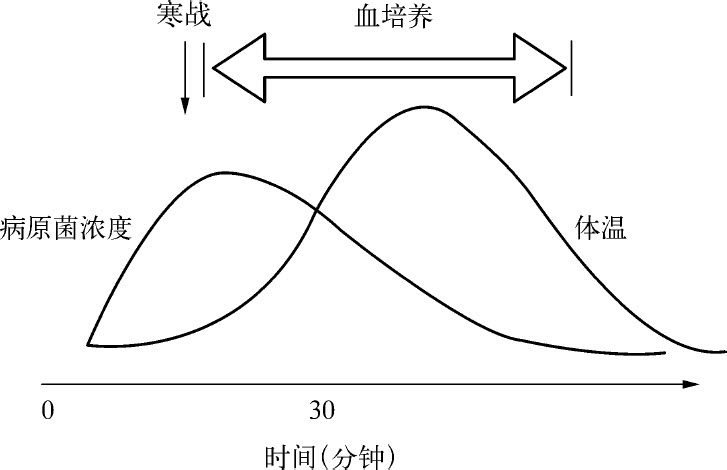
\includegraphics{./images/Image00291.jpg}
 \captionsetup{justification=centering}
 \caption{患者寒战后体温与细菌浓度的变化关系}
 \label{fig25-2}
  \end{figure} 

(3)各种不同病原体血培养的阳性检出率略有差异,金黄色葡萄球菌在首次血培养即可获得阳性结果的比例较高;而铜绿假单胞菌首次血培养即可获得阳性结果的比例较低。CLSI指南推荐:菌血症的患者行4次血培养,且每次采血量为10ml,可获得90%~95%的阳性检出率;当血培养次数增加到6次时,阳性率可增加至95%~99%。

2010年美国感染病学会制定的粒缺指南推荐至少在两个部位采血进行血培养,存在中心静脉插管者可从中心静脉及外周血管同时采血;无此插管者从两个不同部位采血。

(4)病原体血培养的阳性率与采血体积相关,采血量每增加1ml,阳性率随之增加3%。一般要求总采血量在20~40ml。若患者体重低于40kg,采血体积应低于总血容量的1%(一般人体血容量为70ml/kg)。

血培养时培养皿的孵化时间也同样影响血培养的阳性率,血培养时培养皿的孵化时间达72小时者,可获得96%的阳性率。

\subsubsection{常用的感染监测数据有哪些?}

(1)感染率及调整感染率的计算

感染率的表达方式有两种,即病例(例次)感染率和患者日感染率:

\begin{center}

\includegraphics{./images/Image00292.jpg}
\end{center}

(2)器械相关感染率的计算

\begin{center}

\includegraphics{./images/Image00293.jpg}
\end{center}

(3)器械使用率的计算

\begin{center}

\includegraphics{./images/Image00294.jpg}
\end{center}

\begin{center}

\includegraphics{./images/Image00295.jpg}
\end{center}

\subsubsection{感染患者临床病情分类标准是什么?}

每周一次(时间相对固定),按当时患者的病情进行病情评定,每次评定后记录各等级(A、B、C、D及E级)的患者数,每月统计平均,结合病情严重程度评分调整后的各指标可更准确评价不同月份和医院间的感染率差异(表\ref{tab25-1})。

\begin{table}[htbp]
\centering
\caption{感染患者临床病情分类}
\label{tab25-1}
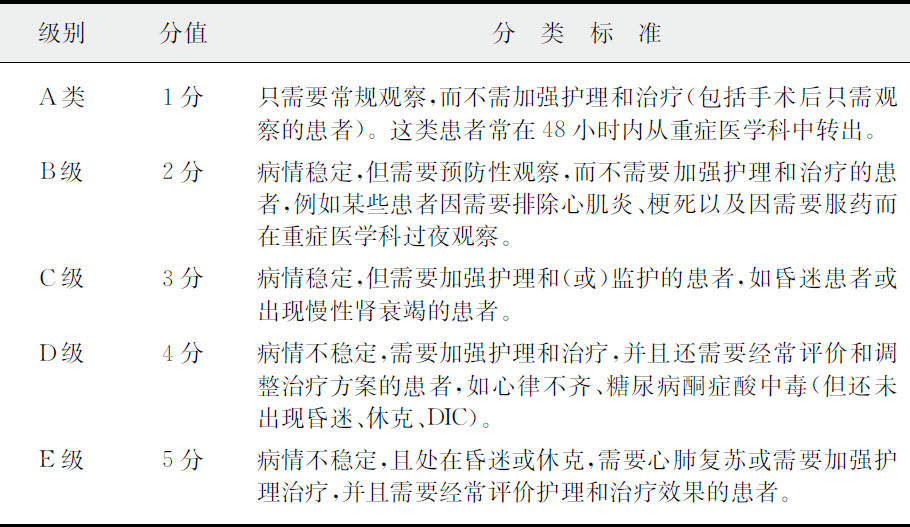
\includegraphics{./images/Image00296.jpg}
\end{table}

\subsection{重症医学科主要院内感染的防控集束化策略}

\subsubsection{重症医学科呼吸机相关性肺炎的防控集束化策略有哪些?}

呼吸机相关性肺炎是指机械通气48小时后发生的肺实质感染性疾病,是一类严重的院内感染。随着重症患者的增多和机械通气的广泛应用,其发病率不断上升。患者一旦发生呼吸机相关性肺炎,平均机械通气时间和住院时间均延长,治疗费用明显增加,治疗困难,患者病死率高达30%左右。预防和控制呼吸机相关性肺炎的发生,是降低机械通气并发症、节约医疗资源和改善重症患者预后的必然要求,应引起重症医学工作者的高度重视。东南大学附属中大医院重症医学科制定了以下医疗工作中需采取的呼吸机相关性肺炎防控措施:

(1)控制环境因素、防止交叉感染 定期对重症医学科病房空气、医护人员、医疗器械和各种装置进行病原菌定植监测,定期进行环境和医疗器械的消毒。医护人员在接触患者前后严格洗手、戴手套和口罩、严格无菌操作,避免手污染和器械污染。

(2)保持患者口腔卫生 加强患者牙齿和口腔清洁,减少口咽部细菌定植。

(3)人工气道气囊压力监测和保持 维持人工气道气囊压力在25~30cm
H\textsubscript{2} O,防止口鼻腔内容物和胃内容物反流和误吸。

(4)声门下吸引 应用带有声门下吸引的人工气道,并保持吸引通畅,减少声门下内容物误吸。

(5)加强呼吸机管路的管理 频繁更换呼吸机管路可能增加呼吸机相关性肺炎的发生,故不需要定期更换呼吸机管道。当管道内有血、呕吐物或呼吸道分泌物时予以更换。防止管路积水杯中冷凝水溢流、及时清除冷凝水。

(6)半卧位 仰卧位是发生呼吸机相关性肺炎的独立危险因素。没有禁忌证的患者,应采取30°的半卧位,既具有临床可操作性,又有利于预防呼吸机相关性肺炎的发生。尤其在进行肠内营养过程中及其之后一段时间,应保持患者处于半卧位。

(7)避免不必要的应激性溃疡预防用药 胃液pH值和胃内细菌检出率显著相关,使用制酸剂后胃液pH值升高,胃内细菌检出率升高。因此对于发生消化道出血危险性低的机械通气患者,尽量避免使用应激性溃疡预防用药;当患者存在应激性溃疡出血的高危因素时,考虑预防用药,优选制酸剂,而不使用硫糖铝。

(8)避免机械通气患者持续镇静 持续镇静及镇静程度过深均增加呼吸机相关性肺炎的发生。对于机械通气患者,应实施每日唤醒的镇静,并进行镇静评分,防止镇静过深。

\subsubsection{中心静脉导管相关血流感染如何判断?}

根据导管是否仍有保留的必要性进行采血检测的方法有两种------保留导管的采血方法为:外周静脉血至少1份,中心静脉血1份;拔除导管的采血及培养方法为:导管血1份、2个不同部位的外周静脉血、导管尖端5cm培养。根据导管是否保留及相应血培养的结果进行导管相关血流感染的判断方法见表\ref{tab25-2},表\ref{tab25-3}。

\begin{table}[htbp]
\centering
\caption{保留导管者结果判读}
\label{tab25-2}
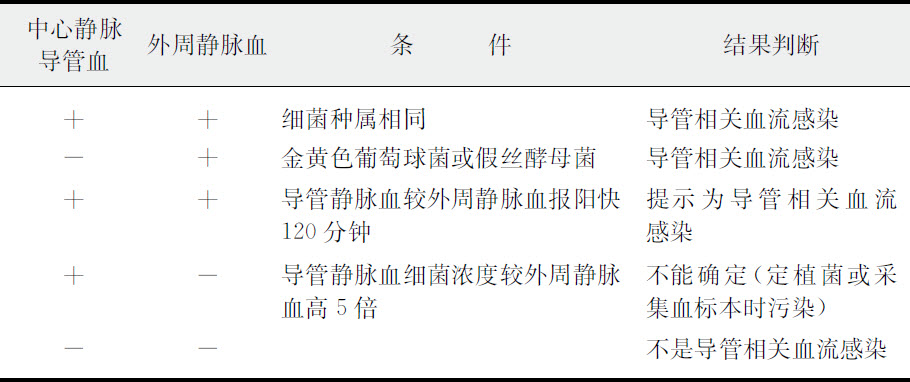
\includegraphics{./images/Image00297.jpg}
\end{table}

\begin{table}[htbp]
\centering
\caption{拔除导管结果判读}
\label{tab25-3}
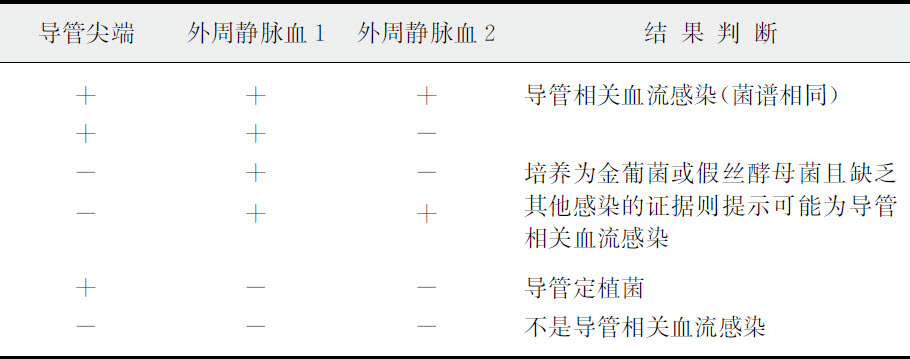
\includegraphics{./images/Image00298.jpg}
\end{table}

\subsubsection{血管内导管相关感染防控的集束化策略有哪些?}

对于重症患者,血管内置管往往不可或缺,成为快速输液、应用血管活性药物、进行血流动力学监测、静脉营养支持以及血液净化的重要途径。但由于本身病情的严重性、皮肤黏膜的破坏、长时间的保留导管等,血管内导管相关感染,尤其血管内导管相关血行感染也随之发生,延长了患者住院时间,增加患者的病死率,加重医疗负担。预防和控制血管内导管相关感染是降低血管内导管使用并发症、节约医疗资源和改善重症患者预后的必然要求,应引起重症医学工作者的高度重视。结合国外研究,东南大学附属中大医院重症医学科制定了医疗工作中需采取的集束化的血管内导管相关感染防控措施:

(1)反复的教育培训,提高防护意识 平时加强医护人员的反复教育,并每年针对新入科室人员进行感染控制的强化培训。

(2)建立中心静脉置管操作规范与核查表 经过培训合格确认有资质的医师才可进行独立置管操作。在每次操作前填写中心静脉穿刺置管术操作与监测记录单。

(3)严格手卫生,督查与考核 在行各种操作,尤其与血液相关的,严格进行洗手和卫生手消毒。不定期检查手卫生的依从性。

(4)置管时采取最大的无菌屏障 行血管内置管时,医生洗手后穿无菌隔离衣,戴帽子、口罩、手套,穿刺点周围15cm严格消毒,周边加铺大的无菌治疗巾。

(5)非隧道式导管穿刺点选择尽量避免股静脉 除紧急情况或患者体位受限,非隧道式中心静脉导管穿刺点选择尽量避免股静脉置管。

(6)专人每日导管护理,每日评估留管的必要性,及时拔除不必要的导管 每日评估导管局部情况以及导管功能、留置的必要性,及时拔除不必要的导管。

(7)皮肤消毒 采用碘伏消毒皮肤,并注意待干后再行穿刺。如有条件优选2%洗必泰液。

(8)严格接口消毒 当接口打开时采用碘伏或70%乙醇严格消毒,尽量减少接口开放的次数。

(9)采用分隔膜式输液接头,减少回血 采用分隔膜式输液接头,并间断冲洗管路,减少回血,降低感染率。

\subsubsection{深静脉置管操作规范是什么?}

(1)经过培训考核合格,取得深静脉置管资质的医生方可独立进行此项操作。

(2)置管前须明确深静脉置管的适应证,排除禁忌证。适应证包括:①需要开放静脉通路,但又不能经外周置管者;②需要多腔同时输注几种不相溶药物者;③需要输注有刺激性或高渗性药液者;④需要血流动力学监测的危重患者;⑤需要为快速容量复苏提供充分保障的患者;⑥进行血液净化、放置肺动脉漂浮导管和临时起搏器。

本操作无绝对禁忌证,相对禁忌证有:①肝素过敏;②穿刺部位感染;③严重凝血功能障碍;④溶栓患者。

(3)置管前准备工作内容有:①签署知情同意书;②常规器械和物品准备,包括一次性消毒包、碘伏、无菌手套、导管包、大的(面积)无菌单、利多卡因、肝素水(浓度)、治疗车、测压装置;③在能满足管理患者需要的前提下,中心静脉导管的端口或者腔道应尽量少;导管留置时间预计超过5天的患者,如果成功地实施了感染控制综合措施仍不能降低导管相关血流感染的发生率,可使用含洗必泰/磺胺嘧啶银或者米诺环素/利福平浸渍的中心静脉导管;④术前适当镇静镇痛;⑤在推荐部位放置中心静脉导管时,相对于机械性并发症(如气胸、锁骨下动脉破裂、锁骨下静脉破损、锁骨下静脉狭窄、血胸、血栓、空气栓塞以及导管错位),应权衡利弊从而减少感染性并发症;应避免使用股静脉作为成人中心静脉通路,对于血液透析患者和终末期肾病患者避免使用锁骨下静脉作为穿刺部位,以免发生锁骨下静脉狭窄;⑥术前清洗穿刺点;⑦颈内或锁骨下静脉穿刺时降低呼吸机呼气末正压水平。

(4)穿刺步骤:①术前洗手、戴口罩、帽子、手套,严格执行无菌操作;②使用碘伏或70%乙醇消毒,有条件时使用浓度大于0.5%的洗必泰消毒术区皮肤,应等消毒剂充分干燥后再穿刺,碘伏消毒需待干2分钟;③最大化无菌屏障措施,在佩戴帽子、口罩、无菌手套的基础上穿无菌手术衣,并全身覆盖无菌消毒巾;④局部浸润麻醉,试穿;⑤静脉穿刺,确认穿刺针尖在中心静脉内------将钝头传感探头通过穿刺针阀门或将针筒脱开针头,如有搏动血流常提示穿入动脉(两种判断标准);或接换能器观察压力波形来判断;⑥以Seldinger法置入导管,确定置入深度,肝素水冲洗导管并封管;⑦妥善固定导管,有条件时使用免缝合装置固定装置;⑧选择适当敷料覆盖穿刺点,若患者易出汗或插管部位有出血或渗出,应首选纱布,不要在插管部位使用抗生素药膏或乳膏;⑨手术后处理(器械处理;利器处理;医疗垃圾处理);⑩洗手;⑪书写记录,包括穿刺并发症,开立术后医嘱;⑫颈内静脉和锁骨下静脉置管行床边胸片确认导管深度(导管尖端位于上腔静脉近右心房处)。

\subsubsection{深静脉导管穿刺点护理规范是什么?}

(1)经过培训且有能力进行外周和中心静脉置管和维护的人员从事此操作。

(2)注意手卫生及无菌操作,换敷料前后应执行手卫生程序,维护导管应持续无菌操作。更换导管敷料时可佩戴清洁或无菌手套。

(3)皮肤消毒使用碘伏或70%乙醇,有条件时使用浓度大于0.5%的洗必泰消毒皮肤:以穿刺点为中心使用0.5%碘伏溶液由内向外做圆周状消毒2遍待干2分钟,消毒面积应大于敷贴面积(固定导管于皮肤的装置下易积存血液、污渍应清除干净)。

(4)局部应覆盖无菌纱布、无菌透明贴膜、半透性敷料。无菌纱布宜选8层,大小为8cm×10cm,患者多汗或者置管部位有出血或渗出时,应使用纱布直到问题解决。

无菌透明贴膜的粘贴方法为:穿刺点周围皮肤处于伸展状态,贴膜中心置于穿刺点上方,向四周平压。颈内静脉留置导管的患者应嘱其头部偏向对侧,股静脉置管的患者,应保持同侧肢体外展45°,减少局部皮肤皱褶,增加透明贴膜与皮肤结合的紧密度,以减少粘贴后的不适感或局部形成张力性水泡。

去除贴膜时,一手指压穿刺点,另一手由贴膜外侧向外方向撕开,使贴膜松动,然后沿导管方向从穿刺点的远心端向近心端揭除贴膜,避免导管移动滑出。

(5)敷料更换时间:①纱布每2日更换一次;②贴膜每周更换1次;③当置管部位敷料潮湿、松弛或者有明显污染时应及时更换。

(6)每天动态观察有无穿刺点局部感染症状(导管入口处红肿、触痛、硬结、有脓性分泌物或弥漫性红斑)及全身症状,如有异常应及时汇报处理并记录。

(7)每天评价导管留置的必要性,达到治疗目的、病情允许后应尽早拔除中心静脉导管,缩短导管留置时间。

\subsubsection{深静脉导管输注装置管理规范是什么?}

(1)医务人员操作前后应洗手或消毒双手。

(2)连续使用的输注装置的更换时间:①不输注血液、血液制品或脂肪乳者4~7天更换一次。②输注血液、血液制品或脂肪乳者,输液开始后的24小时内更换,输注丙泊酚时每6~12小时更换输液瓶时更换输液管。

(3)接口使用前用0.5%碘伏消毒2次,然后再连接输液器;局部区域清洁可用无菌巾包裹,24小时更换一次,污染后及时更换;应减少不必要的附加装置,避免不必要的断开管路。

(4)使用静脉药物前注意检查药液的质量及有效期,不符要求者不得使用。

(5)输液过程中,应保持导管通畅。每次输液前应先抽回血,见回血后方可接上输液,输液过程加强巡视,防止导管受压、打折或输液器与导管接头脱开。

(6)尽量避免自中心静脉导管采血和输血。

(7)每日输液结束后先用生理盐水5~10ml冲洗管腔,再用12.5U/ml肝素钠盐水做脉冲式封管;但对于有些不宜用肝素的疾病及对肝素过敏者可使用生理盐水封管;封管时不要抽回血,关闭水止阀时支点位于注射器侧,避免接触患者侧,以免接触导管形成正压,离开后回血至导管内。

(8)导管脱出后勿再送入血管,并做好标记。

(9)中心静脉置管深度、通畅与否等作为交接班的内容记录。

\subsubsection{重症医学科导尿管相关泌尿系统感染的防控策略是什么?}

(1)严格掌握留置导尿的适应证,减少不必要插导尿管及不必要延长留置时间 留置导尿管的适应证为:①解除尿路阻塞;②允许神经源性膀胱功能失调和尿潴留的患者导尿;③泌尿道手术或生殖道手术的患者;④危重患者需要准确记录尿量。

如病情评估允许优先选择非侵入操作式导尿,行非侵入引留尿液与植入导尿管序贯治疗方法相结合,必要时插入导尿管。

不适宜留置导尿管的情况包括:①患者能够自主排尿;②仅为获得尿培养或某种诊断检查如尿电解质而采集尿标本;③对尿失禁患者安置留置导尿管而代替一般护理;④急性尿道炎,急性前列腺炎,急性附睾炎,月经期为其禁忌证。

(2)留置导尿的宣教 其内容包括:①对患者、家属、护工进行宣教;②对医护人员进行教育培训,规范诊疗过程监控、危险因素管理,全方位进行感染预防控制;③控制导尿管感染危险因素;④定期分析导尿管相关泌尿系感染发病率,用数据推行感染预防制度的完善与推行,达到全员参与感染控制。

(3)按照导尿管操作常规执行尿管留置 ①要求只有掌握无菌插管正确技术和导管护理的人员(如医院工作人员、家属或患者)才能操作导管;②应用无菌技术和无菌器材插管和护理导尿管;③维持持续的密闭无菌引流系统。

(4)采尿标本和更换导尿管频率 ①菌尿症不推荐频繁监测。每周常规做一次尿常规检查,如有尿路感染时及时采集标本做尿常规和细菌培养评估感染发生,指导诊治。尿液标本在室温下放置不能超过2小时,应及时送检微生物检验接种。②对于长期留置导尿管的患者,建议每4~6周更换导尿管;当患者有尿路感染征象时,在开始使用抗菌药物治疗之前就先更换导尿管,对降低留置导尿管相关尿路感染的效果较好。

(5)不推荐使用的处理方法 ①膀胱冲洗:除非患者病情需要,否则应避免膀胱冲洗。定期使用生理盐水、抗菌药物或消毒剂膀胱冲洗并不能降低导尿管相关尿路感染的发生率;②全身应用抗菌药物预防导尿管相关泌尿系感染。

(6)膀胱功能训练与评估 由患者自己控制,当有尿意时放开尿管,流尽尿液后再夹闭尿管,如此反复以训练膀胱收缩功能,促进及早拔管,可结合原发病治疗恢复情况决定拔管。

(7)尿管相关尿路感染的预防 插管前准备与插管时的措施包括:①尽量避免不必要的留置导尿;②仔细检查无菌导尿包,如过期、外包装破损、潮湿,不得使用;③根据年龄、性别、尿道情况选择合适的导尿管口径、类型。通常成年男性选16F,女性选14F;④规范手卫生和戴手套的程序;⑤尽可能选择单包装的灭菌润滑剂;⑥常规用0.25%~0.5%碘伏消毒尿道口及其周围皮肤黏膜------男性自尿道口、龟头向外旋转擦拭消毒,注意洗净包皮及冠状沟;女性先清洗外阴,其原则由上至下,由内向外,然后清洗尿道口、前庭、两侧大小阴唇,最后会阴、肛门,每一个棉球不能重复使用;⑦插管过程严格执行无菌操作,动作要轻柔,避免尿道黏膜损伤;⑧对留置导尿患者,应采用密闭式引流系统。

插管后的预防措施包括:①保持尿液引流系统通畅和完整,不要轻易打开导尿管与集尿袋的接口;如要留取尿标本,可从集尿袋采集,但此标本不得用于普通细菌和真菌学检查;②导尿管不慎脱落或导尿管密闭系统被破坏,需要更换导尿管;③集尿袋不得高于膀胱水平,也不可接触地面,如下床活动或搬运时,应临时夹闭并固定尿袋引流管,防止反流;④集尿袋达2/3满时要及时排放,放尿时尿袋末端管口防止污染;疑似导尿管阻塞应更换导管,不得冲洗;⑤不应常规采用膀胱冲洗预防泌尿道感染;⑥保持会阴部清洁干燥;⑦尿路感染使用抗菌药物前,应送尿培养,必要时拔除导尿管;⑧长期留置导尿患者,导尿管更换1次/2周,集尿袋更换1次/2周,更换时注意无菌操作;⑨每日评价留置导管的必要性,尽早拔除导尿管;⑩长期留置导管患者,建议每周检测尿常规一次;⑪定期对医务人员进行宣教,每月公布导尿管相关尿路感染发生率。

\begin{center}\rule{0.5\linewidth}{\linethickness}\end{center}

参考文献

\protect\hyperlink{text00031.htmlux5cux23ch1-30-back}{{[}1{]}}
.Harrington G,Watson K,Bailey M,et al.Reduction in hospitalwide
incidence of infection or colonization with methicillin-resistant
Staphylococcus aureus with use of antimicrobial hand-hygiene gel and
statistical process control charts.Infect Control Hosp
Epidemiol,2007;28(7):837-844.

\protect\hyperlink{text00031.htmlux5cux23ch2-30-back}{{[}2{]}} .Lederer
Jr JW,Best D,and Hendrix V.A comprehensive hand hygiene approach to
reducing MRSA health care-associated infections.Jt Comm J Qual Patient
Saf,2009;35(4):180-185.

\protect\hyperlink{text00031.htmlux5cux23ch3-30-back}{{[}3{]}} .O'Grady
NP,Alexander M,Burns LA,et al.Guidelines for the Prevention of
Intravascular Catheter-related Infections.Clin Infect
Dis,2011;52:e162-e193.

\protect\hyperlink{text00031.htmlux5cux23ch4-30-back}{{[}4{]}} .Hooton
TM,Bradley SF,Cardenas DD,et al.Diagnosis,Prevention,and Treatment
of Catheter-Associated Urinary Tract Infection in Adults:2009
International Clinical Practice Guidelines from the Infectious Diseases
Society of America.Clin Infect Dis,2010;50:625-663.

\protect\hyperlink{text00031.htmlux5cux23ch5-30-back}{{[}5{]}}
.Nachtigall I,Tamarkin A,Tafelski S,et al.Impact of adherence to
standard operating procedures for pneumonia on outcome of intensive care
unit patients.Crit Care Med,2009;37(1):159-166.

\protect\hyperlink{text00031.htmlux5cux23ch6-30-back}{{[}6{]}}
.陈佰义,何礼贤,胡必杰,倪语星,邱海波,石岩,施毅,王辉,王明贵,杨毅,张菁,俞云松.中国鲍曼不动杆菌感染诊治与防控专家共识.中华医学杂志,2012;92(2):76-85

\protect\hyperlink{text00031.htmlux5cux23ch7-30-back}{{[}7{]}}
.Tschudin-Sutter S,Pargger H and Widmer AF.Hand hygiene in the
intensive care unit.Crit Care Med,2010;38(8 Suppl):S299-305.

\protect\hyperlink{text00031.htmlux5cux23ch8-30-back}{{[}8{]}} .Coia
JE,Duckworth GJ,Edward DI,et al.Guidelines for the control and
prevention of meticillin-resistant Staphylococcus aureus(MRSA)in
healthcare facilities.J Hosp Infect,2006;63 Suppl 1:S1-44.

\protect\hyperlink{text00031.htmlux5cux23ch9-30-back}{{[}9{]}}
.Markogiannakis A,Fildisis G,Tsiplakou S,et al.Cross-transmission
of multidrug-resistant Acinetobacter baumannii clonal strains causing
episodes of sepsis in a trauma intensive care unit.Infect Control Hosp
Epidemiol,2008;29(5):410-417.

\protect\hyperlink{text00031.htmlux5cux23ch10-30-back}{{[}10{]}}
.Falagas ME and Karageorgopoulos DE.Pandrug
Resistance(PDR),Extensive Drug Resistance(XDR),and Multidrug
Resistance(MDR)among Gram-Negative Bacilli:Need for International
Harmonization in Terminology.Clin Infect Dis,2008;46:1121-1122.

\protect\hyperlink{text00031.htmlux5cux23ch11-30-back}{{[}11{]}}
.李春辉摘译,吴安华审校.医疗机构耐药菌MDR、XDR、PDR的国际标准化定义专家建议(草案).中国感染控制杂志,2011;10(3):238-240

\protect\hyperlink{text00031.htmlux5cux23ch12-30-back}{{[}12{]}}
.Magiorakos AP,Srinivasan A,Carey RB,et
al.Multidrug-resistant,extensively drug-resistant and
pandrug-resistant bacteria:an international expert proposal for interim
standard definitions for acquired resistance.Clin Microbiol
Infect,2012;18(3):268-281.

\protect\hyperlink{text00031.htmlux5cux23ch13-30-back}{{[}13{]}}
.Freifeld AG,Bow EJ,Sepkowitz KA,et al.Clinical Practice Guideline
for the Use of Antimicrobial Agents in Neutropenic Patients with
Cancer:2010 Update by the Infectious Diseases Society of America.Clin
Infect Dis,2011;52:e56-e93.

\protect\hyperlink{text00031.htmlux5cux23ch14-30-back}{{[}14{]}} .Towns
ML,Jarvis WR,and Hsueh PR.Guidelines on blood cultures.J Microbiol
Immunol Infect,2010;43(4):347-349.

\protect\hypertarget{text00032.html}{}{}

